\section{Sistema de Refrigeração}
A refrigeração da câmara tem como base o uso da pastilhas termo elétricas, denominadas de módulos Peltier que são pequenas unidades que utilizam tecnologia de matéria condensada para operarem como bombas de calor. Esta pastilha é feita de material semicondutor e é capaz de causar um diferença de temperatura nas suas faces quando submetida à uma tensão.

\subsection{Estrutura do conjunto de refrigeração}
Pelas especificações do projeto em ser um ambiente de refrigeração para o transporte de órgãos para transplante, a face de menor temperatura da célula peltier deve estar em contato com o ar de dentro da câmara para que assim ocorra o seu resfriamento. Já o lado de maior temperatura da célula peltier deve estar em contato com o ar circundante no ambiente externo, tornando assim a troca de calor entre as duas regiões mais eficaz.

Em vista disso, serão utilizados dois dissipadores de calor, que estarão em contato direto com uma pasta térmica, e esta irá em contato com o módulo peltier. Logo acima das colmeias de cada dissipador haverá um cooler, que tem como principal objetivo melhorar a circulação de ar pelos dissipadores, consequentemente tornar a troca de calor do sistema ainda mais eficiente.

Na figura abaixo é apresentada uma visão explodida da solução de refrigeração:

\begin{figure}[H]
\begin{center}
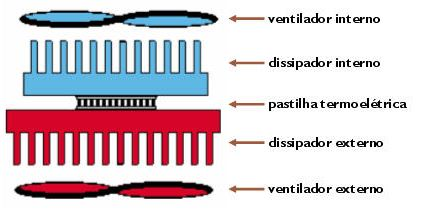
\includegraphics[scale = 1]{figuras/Sistema_Ref.JPG}
\caption{Visão explodida do sistema de refrigeração}
\end{center}
\end{figure}

O desempenho dos módulos peltier é diretamente proporcional às grandezas que o controlam. Devido a esta característica, para um projeto o fabricante disponibiliza um conjunto de curvas que irão permitir ao projetista determinar os limites seguros de operação do sistema de refrigeração. Algumas combinações dessas grandezas podem tornar o sistema que possui um comportamento ótimo para um desempenho inadmissível. 

\begin{table}[H]
\begin{center}
\caption{Dados de Desempenho da Célula Peltier. FONTE: Folha de Dados TEC-12706 – HB Eletronic Components.}
\begin{tabular}{|c|c|c|}
\hline
\textbf{Temperatura do lado quente (ºC)} & 25 & 50  \\
\hline
\textbf{$Q_{MAX}$ (W)} & 50 & 57 \\
\hline
\textbf{$\Delta T_{MAX}$ (ºC)}& 66 & 75 \\
\hline
\textbf{$I_{MAX}$ (A)} & 6,4 & 6,4 \\
\hline
\textbf{$V_{MAX}$ (V)} & 14,14 & 16,4 \\
\hline 
\textbf{Resistência do Módulo ($\Omega$)} & 1,98 & 2,3\\
\hline
\end{tabular}

\end{center}
\end{table}
\subsection{Dimensionamento do sistema de refrigeração Peltier}
O dimensionamento do sistema de refrigeração por Peltier irá ser desenvolvido de modo sistemático, tendo como referência a definição de uma carga térmica e a diferença de temperatura quente/frio (DT) [1]. Cabe alertar que serão determinados pontos ótimos de operação e uma estimativa de desempenho para o sistema uma vez que o sistema tem um comportamento não-linear. 

\subsubsection{Determinação das temperaturas de trabalho}
Serão definidas nesta etapa as temperaturas de trabalho, afim de:
\begin{itemize}
	\item Fazer a escolha do módulo peltier;
    \item Escolher o dissipador de calor para o módulo;
    \item Calcular as cargas térmicas do projeto. 
\end{itemize}
Portanto, as temperaturas de trabalho estão assim estabelecidas:
\begin{table}[H]
\caption{ Temperaturas de trabalho do módulo Peltier}
\begin{tabular}{c|c|c}
     &  \textbf{Temperatura (ºC)} & \textbf{Observação}\\
   \hline
   $T_{ambiente}$ & 35 & Temperatura ambiente em que o dispositivo vai trabalhar \\
   $T_Q$ & 40  & 
Temperatura de trabalho da face quente - dissipador \\
$T_F$ & 0 & Temperatura de trabalho da face fria \\
$\Delta T$ & 40 & 
Os limites do módulo estão ligados a esta variável\\
\hline
\end{tabular}
\end{table}

\subsubsection{Determinação da Carga Térmica}
Existem dois tipos de carga térmica que o sistema de refrigeração vai estar submetido, a carga térmica ativa que é a energia térmica dissipada pelo dispositivo que estará sendo refrigerado, e a carga térmica passiva, a qual é a energia térmica proveniente de radiação, convecção ou condução, ou ainda a combinação dos dois. 

\begin{equation}
Q_{Térmica} = Q_{Radiação}+Q_{Condução}+Q_{Convecção}+Q_{Ativa}
\end{equation}
Descobrir e minimizar as cargas térmicas atuantes no sistema nos permitirá alcançar o nível de refrigeração requisitado e a potência necessária para alcançá-la. A seguir serão estimadas as cargas ativa e passiva do sistema.
\begin{itemize}
\item Carga Térmica Ativa

Esta  fonte é relacionada à presença de dispositivos, no caso em questão à presença do cooler, na região a ser refrigerada e esta carga é representada pela potência dissipada por efeito Joule:
\begin{equation}
Q_{Ativa} = V \times I
\end{equation}
Onde:

$Q_{Ativa}$ --- Potência ativa, em Watts;

V --- Tensão de alimentação do dispositivo (12 V);


I --- Corrente no dispositivo (0,15 A).

O que leva a concluir que a carga térmica ativa é de aproximadamente 1,8 Watts.

\item Carga Térmica Passiva

Para este projeto o cálculo da carga térmica de radiação será desprezado, pois o sistema não trabalha com altas temperaturas à vácuo.

Para o cálculo da carga térmica passiva será utilizada a combinação dos fenômenos de condução e convecção:
\begin{equation}
	Q_{Passivo}= \frac{A \times \Delta T}{\frac{x}{k} + \frac{1}{h}}
\end{equation}
Para o cálculo da área externa foram utilizadas as dimensões externas da câmara de $6\times(300 \times 300)\times 10^{-6}=0,54mm^2$. 

Considerando duas possibilidades de isolantes térmicos que podem ser utilizados no projeto (Poliestireno Expandido e Espuma de Poliuretano), obtêm-se:

Poliestireno expandido (EPS) --- Isopor: 0,045 a 0,034 $\left[\frac{W}{m.K}\right]$ e espessura x=0,02m.

Espuma de poliuretano: 0,023$\left[\frac{W}{m.K}\right]$ e espessura 0,03 m.

Foi utilizado o coeficiente de transferência de calor por convecção do ar por convecção forçada: $h = 250 \left[\frac{@}{M^2.ºC}\right] $

Obtendo assim, duas cargas térmicas passivas:

$Q_{Passiva, Isopor}$ = 24,73 W

$Q_{Passiva, Espuma} $ = 26,51 W

Como as duas cargas são comparativamente próximas, para fins práticos de cálculo será escolhida a maior dentre elas.

Logo, $Q_{Térmica}$ = 28,31 W.

\end{itemize}

\subsubsection{Determinação de Estágios para o Módulo}
Com base nas definições de temperaturas realizadas anteriormente, pode-se determinar portanto o número de estágios do módulo necessários para que o $\Delta T$ seja atingido com segurança.

Com base nas definições de temperaturas realizadas anteriormente, pode-se determinar portanto o número de estágios do módulo necessários para que o T seja atingido com segurança.

\begin{table}[H]
\begin{center}
\caption{Diferença máxima de temperatura para módulos simples e de dois e três estágios}
\begin{tabular}{c||c}
\textbf{Número de Estágios} & \textbf{$\Delta T Max$} 1 atm de $N_2$\\
\hline \hline
1 & 64\\
2 & 84 \\
3 & 95\\
\hline \hline
\end{tabular}
\end{center}
\end{table}

\subsubsection{ Escolha da Célula de Peltier}
Com base no método dimensionamento por carga térmica, é necessária uma célula de Peltier de 28,31  W para climatizar um compartimento de transporte.

Para esse projeto então, será utilizada para fazer a função de climatização do compartimento de transporte de órgãos uma célula de Peltier, cujo modelo adotado foi o TEC1-12706, por ser de fácil acesso no mercado e suprir as necessidades do projeto, conforme os cálculos de dimensionamento por carga térmica realizados. Este modelo possui comprimento e largura de 4cm e altura de 3,2mm. A corrente elétrica máxima que esta célula de peltier pode suportar é de 6 Ampères, a tensão máxima é de 15,4V e a potência máxima é de 63W. 

\subsubsection{Controle do Cooler}

Para controlar a velocidade do cooler será utilizado um controle PWM de forma em que o tempo em que a onda fica em nível lógico alto em relação a todo o período da onda determina a porcentagem de potência entregue ao sistema, e forma a ajustar o consumo de energia para evitar que o consumo de energia seja muito alto desnecessariamente.

\subsubsection{Controle da Célula Peltier}

Da mesma forma que  o cooler o consumo do peltier será estimado pelo controle via PMW, como no caso do peltier se faz necessário o uso de uma tensão de 12V será usado um controle de interrupção simples utilizando transistor MOSFET para atuar como chave que será controlada pelo próprio PWM.

\subsection{Requisitos do Sistema}

Com vistas à concepção e validação da solução, foram definidos os requisitos relativos ao subsistema de alimentação e refrigeração do produto:

\subsubsection{Requisitos Funcionais}
O sistema de refrigeração deve ser capaz de:
\begin{itemize}
\item Refrigerar uma câmara hermeticamente;
\item sistema deve ser capaz de estabilizar a temperatura interna da câmara de forma que o órgão fique com temperatura entre 2ºC e 4ºC;
\item O sistema deve ser capaz de manter a temperatura da câmara uniforme.

\end{itemize}
\subsubsection{Requisitos Não-Funcionais}
O sistema de refrigeração deve ser capaz de:
\begin{itemize}
\item Utilizar dissipadores de calor e células de peltier;
Ser eficiente energeticamente, consumindo o mínimo de consumo possível através de um controle de potência;
\item A câmara a ser refrigerada deve ter um volume máximo de 4 litros;
\item O sistema deve ser capaz de refrigerar o sistema de forma satisfatória durante um período máximo de 48 horas.
\end{itemize}

\section{Sistema de Alimentação}
As fontes de energia que serão utilizadas para alimentar o produto, incluindo o sistema de refrigeração e os componentes elétricos e eletrônicos, são a rede elétrica comum brasileira e um banco de baterias. O banco de baterias será dimensionada a fim de manter os subsistemas em perfeita operação durante o período solicitado de 48 horas.

\subsection{Diagrama do Sistema}
A Figura a seguir apresenta o diagrama elétrico simplificado do produto. Ele representa o circuito de alimentação utilizado, desde a fonte de energia --- rede elétrica padrão --- até o uso final em seus componentes elétricos e eletrônicos.  É importante ressaltar que este diagrama será refinado ao longo dos pontos de controle, pois o  sistema pode ser retificado para melhor atender às condições de contorno que forem encontradas durante a execução do projeto.

\begin{figure}[H]
\begin{center}
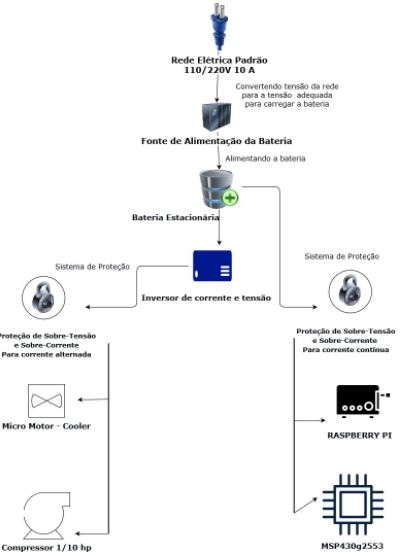
\includegraphics[scale = 1.2]{figuras/Diagrama_Simp.JPG}
\caption{ Diagrama Elétrico Preliminar}
\end{center}
\end{figure}

O sistema foi dimensionado com um fator de segurança elevado, pois a proposta de projeto é de um sistema de acondicionamento de órgãos para transplante. Sendo assim, o nível de confiabilidade do produto deve ser extremamente alto, para isso todo o sistema de alimentação foi dimensionado relacionando o sistema ao tempo de operação necessário ao transporte e diretamente ao consumo de energia advinda da bateria.


\subsection{Dimensionamento das Baterias}
	Baterias têm a finalidade de armazenar energia e liberá-la em determinada periodicidade, e de forma controlada. Sua escolha deve ser adequada às necessidades de consumo energético do projeto, e considera os dados de corrente elétrica e tensão. Para a seleção da bateria adequada deve-se estudar se ela é capaz de armazenar a energia total demandada às necessidades do projeto, e se ela consegue entregar toda a energia necessária ao funcionamento do equipamento. O processo de dimensionamento do banco de baterias deve ser realizado inicialmente e depois sucessivamente aperfeiçoado, em função dos demais dimensionamentos e ajustado em função dos custos, disponibilidade de mercado, entre outros.

	O processo de dimensionamento deve seguir algumas etapas, a primeira delas é definir o tipo de bateria a ser utilizado. Dentre as opções de bateria disponíveis no mercado, optou-se pela bateria estacionária. Sua vida útil é de aproximadamente 5 anos, devido à sua composição com materiais internos mais sobres se comparada às baterias automotivas, por exemplo. Podem, também, suportar descargas de até 80\% de sua capacidade, sem prejudicar sua vida útil, e resistem a ciclos de carga ou descarga mais profundos. Tais características proporcionam maior confiabilidade ao funcionamento do projeto pelo uso da bateria estacionaria.
	
	Após a escolha do tipo de bateria, deve ser analisada a profundidade de descarga com que se vai trabalhar. Quanto mais profundos os ciclos de descarga-carga, menor a vida útil da bateria. Ou seja, reduzir-se a capacidade da bateria, gasta-se menos no início, porém as baterias durarão menos e os gastos com reposição serão maiores. Um valor usado para essa profundidade de descarga para ciclos diários com baterias de chumbo-ácido é de 10\% a 20\%. Para ciclos esporádicos, podem ser utilizados ciclos mais profundos, da ordem de 60\%. 
	
	A capacidade do banco de baterias em Ah pode ser calculada conforme a expressão abaixo: 
	
	\begin{equation}
	Capacidade(Ah) = \frac{Consumo(\frac{Wh}{dia}) \times Autonomia(dias)}{V_{Baterias}(V)\times profundidade(pu)}
	\end{equation}

O dimensionamento da bateria requer inicialmente a relação de potência demandada para suprir as necessidades dos componentes elétricos do projeto, como mostra a tabela a seguir:

\begin{table}[H]
\caption{Consumo energético dos componentes}
\begin{tabular}{|p{4 cm} |c |c |c |}
 \hline
   \textbf{COMPONENTE} &\textbf{ALIMENTAÇÃO (V)}  &\textbf{CORRENTE (A)} & \textbf{POTÊNCIA (W)} \\
   \hline
  \textbf{MSP430g2553} &5 & 330$\mu$& 1,65 mW \\
   \hline
   \textbf{RASPBERRY PI}&5 &2,5 & 12,5 \\
   \hline
  \textbf{PROTETOR } &12 &26,5m &318m \\
   \hline
  \textbf{COMPRESSOR $\frac{1}{10}HP$} &12 & 2,4& 28,33 \\
   \hline
  \textbf{MICRO MOTOR} &12 &260,9m &3,6  \\
   \hline

\end{tabular}
\end{table}

Ao somar todas as cargas necessárias, o total foi de 229,819 Wh, já o consumo de corrente fica em 3,5365 A/h. O principal problema é o alto valor de partida do motor-compressor, o que é chamado de corrente de pico, no caso do motor-compressor utilizado, a corrente pode atingir um o valor entre 2-3 Ampères, o que requer atenção ao dimensionar a bateria para que ela suporte esse aumento inicial.


Com relação a profundidade da descarga no final da autonomia (pu) - utilizamos 0,6 (descargas mais profundas significam vida útil menor para a bateria e menos profundas um investimento inicial maior). Sendo que o consumo total é obtido a partir do levantamento das cargas, a autonomia de 5 horas.

Logo, 
$$
Capacidade \approx 33,2439 Ah
$$


\subsection{Dimensionamento do Inversor}
Inversores são conversores estáticos que, segundo Matakas Jr. E Komatsu (2011) transformam corrente ou tensão de forma contínua para a alternada. Muitos equipamentos operam em corrente/tensão contínua, sendo que a rede elétrica opera em corrente/tensão contínua. Portanto, a maneira mais simples de se trabalhar sem necessidade de mudanças drásticas em nenhum dos dois sistemas é se utilizar um inversor.

Este equipamento pode ser monofásico ou trifásico, sendo que o modelo utilizado no projeto será monofásico, e irá converter 12V da bateria que alimenta o sistema para 220V, valor de tensão que os outros componentes do sistema trabalham. Neste caso, com apenas duas chaves eletrônicas e uma fonte de tensão CC dividida é possível obter o inversor desejado.

Os inversores podem operar com duas tecnologias, senóide modificada ou senóide pura. No primeiro caso, formam uma onda quadrática, aproximando-se da senoidal AC, bom custo x benefício e pode ser aplicado na maioria dos casos, exceto para motores. O segundo caso pode ser usado como suprimento de energia AC em qualquer sistema, o que difere é o valor e o tamanho.

Um inversor bem dimensionado tem a potência maior que o consumo dos equipamentos para evitar que este trabalhe sempre em máxima potência,em suma um inversor é projetado em 3 estágios, oscilador, driver de corrente e transformador.
\begin{figure}[H]
	\begin{center}
		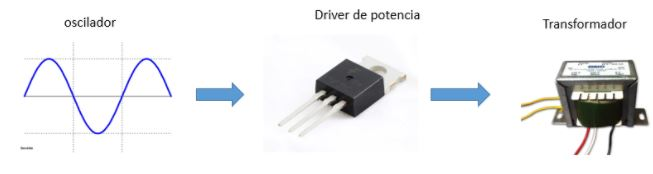
\includegraphics[scale = 0.75]{figuras/dim_inversor.JPG}
		\caption{ Diagrama Elétrico Preliminar}
	\end{center}
\end{figure}

Em primeiro lugar o oscilador transforma a corrente contínua em uma onda quadrada de 60Hz, que precisa ser adequada para uma onda senoidal, para isso é utilizado um filtro passa faixa centrado em 60Hz para eliminar as harmônicas indesejadas e obter uma onda senoidal mais eficaz possível. Entretanto, a saída do oscilador possui uma corrente muito baixa, por isso é necessário um ganho de corrente, para que seja entregue uma potência satisfatória na entrada do primário do transformador. Como a potência requerida é muito alta, se faz necessário que sejam inseridos vários transistores em paralelo para aumentar o ganho de corrente.

Na última fase o transformador faz a elevação da tensão para 220V que é a tensão necessária para ligar o compressor.

\subsection{Requisitos}
Com vistas à concepção e validação da solução, foram definidos os requisitos relativos ao subsistema de alimentação e refrigeração do produto:

\subsubsection{Requisitos Funcionais}
O sistema de alimentação deve ser capaz de:
\begin{itemize}
\item Armazenar energia elétrica;
 \item Fornecer energia para os componentes elétricos e eletrônicos de controle e monitoramento do produto;
 \item Fornecer energia para o sistema de refrigeração.
 \end{itemize}
\subsubsection{Requisitos Não Funcionais}
O sistema de alimentação deve ser capaz de:
\begin{itemize}
\item Prover a energia necessária para o bom funcionamento do produto durante um período máximo de 48 horas, com armazenamento de energia em baterias;
\item O sistema deve ser capaz de controlar a potência que será entregue as placas de peltier;
 \item Possuir eficiência energética aceitável, através de um controle de potência no sistema de refrigeração, escolha de componentes eletrônicos de baixa potência e sistemas de standby em determinados componentes não críticos do produto;
 \item Ser estável energeticamente, evitando picos de potência com componentes e segurança de circuitos.
 \end{itemize}